\documentclass{article}
\usepackage{graphicx} % Required for inserting images
\usepackage{amsmath}
\usepackage{enumitem}
\usepackage[paper=a4paper, margin=2cm]{geometry}
\usepackage{eurosym}
\usepackage{xcolor}
\usepackage{float}
\usepackage{pgfplots}

\title{Algorithmic Methods for Mathematical Models\\
  Course Project }
\author{Tim Wichelmann\\ \texttt{tim.wichelmann@estudiantat.upc.edu}\\[1ex] % [1ex] adds vertical space
  Jakob Eberhardt\\ \texttt{jakob.eberhardt@estudiantat.upc.edu}}
\date{\today}

\begin{document}

\maketitle

\section{Formal Problem Statement}

Time slots are from 1 to $t$.
Orders are numbered 1 to $n$.

We have as inputs the following variables:
\begin{itemize}
    \item $profit_i$ : profit in \euro{ } that we make if order i is taken.
    \item $length_i$ : number of time slots required for baking order i.
    \item $min\_deliver_i$ : earliest time slot the customer could pick up order i.
    \item $max\_deliver_i$ : latest time slot the customer could pick up order i.
    \item $surface_i$ : surface in the oven that order i requires, measured in $m^2$.
\end{itemize}
Orders have to be picked up at the same time slot as the baking process finishes. 
Moreover, the oven in the bakery has a limited surface capacity of surface capacity $m^2$.
At any time, the total surface of the bread that is being baked cannot exceed this capacity.

The goal is to maximize the profit made with the choice of the orders we take.

\section{Integer Linear Programming Model}

%%% TODO: Inlcude input data as PDF suggests %%%

\subsection{Decision variables}
\begin{itemize}
    \item $y_{ij}$ is a matrix of binary variables which indicates if the order $i$ is being baked in time slot $j$.
\end{itemize}

\subsection{Auxiliary variables}

\begin{itemize}
\item $x_i$ is a binary variable indicating whether order $i$ has the right amount of time slots assigned to it. 
We use it as an indicator of 
% \item $\mathit{start}_{ij}$ denotes the time slot $j$ in which the baking process of order $i$ is started.
\item $\mathit{start}_{i}$ denotes the time slot in which the baking process of order $i$ is started.
\end{itemize}

\subsection{Objective function}

\begin{equation*}
  \max \sum^n_{i = 1} \mathit{profit}_i \: x_i
\end{equation*}

\subsection{Constraints}

Subject to
\begin{enumerate}
 %    \item Every processed order has finished baking before the maximum delivery time: 
 %    \begin{equation}
 %    \mathit{start}_{ij}(j + \mathit{length}_i - 1) \leq \mathit{max\_deliver}_i, (1 \leq i \leq n, 1 \leq j \leq t)
 %    \end{equation}
 %    \item Every processed order has finished baking after the minimum delivery time:
 %    \begin{equation}
 %        j + \mathit{length}_i - 1 \geq \mathit{start}_{ij} \: \mathit{min\_deliver}_i, (1 \leq i \leq n, 1 \leq j \leq t) 
 %    \end{equation}
    \item In every time slot, the space capacity is respected:
    \begin{equation}
        \sum^n_{i=1}\mathit{surface}_i \: y_{ij} \leq \mathit{surface\_capacity}, (1 \leq j \leq t)
    \end{equation}
 %    % \item The auxiliary variable $\mathit{start}_i$ has the intended meaning:
 %    % \begin{equation}
 %    %     \mathit{start}_i \leq \mathit{max\_deliver}_i - \mathit{length}_i
 %    % \end{equation}
    % \item We assign the correct amount of time slots or zero time slots to every order:
    % \begin{equation}
    %     \sum^t_{j = 1} y_{ij} = x_i \: \mathit{length}_i, (1 \leq i \leq n)
    % \end{equation}
 %    \item The time slots assigned to this order are contiguous (If an order $i$ starts in time slot $j$, it occupies the consecutive time slots from $j$ to $j + length_i$:
 % %%   \begin{equation}
 % %%       \mathit{start}_{ij} = 1 \doublearrow \sum^{j+\mathit{length}_i-1}_{k=j} y_{i,k} = \mathit{length}_i 
 % %%   \end{equation}
 %        \begin{equation}
 %        \sum^{j+\mathit{length}_i-1}_{k=j} y_{i,k} \geq \mathit{start_}{ij} \mathit{length}_i, (1 \leq i \leq n, 1 \leq j \leq t - \mathit{length}_i + 1 )
 %    \end{equation}
 %    \item Each order only has one start point:
 %    \begin{equation}
 %    \sum^{t}_{j = 1} \mathit{start}_{ij} = x_i, (1 \leq i \leq n)
 %    \end{equation}
     \item We assign the correct amount of time slots or zero time slots to every order:
    \begin{equation}
        \sum^{\mathit{max\_deliver}_i}_{j = \mathit{min\_start}_i} y_{ij} = x_i \: \mathit{length}_i, (1 \leq i \leq n)
    \end{equation}
    \item There are no orders assigned to their respective infeasible slots:
        \begin{align}
	  \sum_{j = 1}^{\mathit{min\_start}_i-1} y_{ij} &= 0, (1 \leq i \leq n) \\
	  \sum_{j = \mathit{max\_deliver}_i+1}^t y_{ij} &= 0, (1 \leq i \leq n)
        \end{align}

        \item Each order is started in on of the feasible time slots.
        \begin{align}
                	forall(i in N)
	  start[i] <= max_start[i];
    forall(i in N)	
	  min_start[i] <= start[i];    
        \end{align}

        \item Contiguous
\end{enumerate}


\begin{figure}[H]
\centering
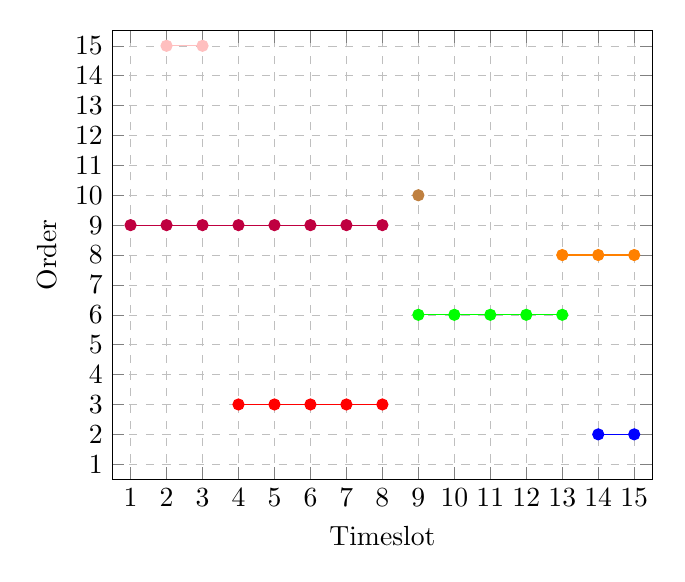
\begin{tikzpicture}
\begin{axis}[
    title={},
    xlabel={Timeslot},
    ylabel={Order},
    xmin=0.5, xmax=15.5, 
    ymin=0.5, ymax=15.5, 
    xtick={1,2,3,4,5,6,7,8,9,10,11,12,13,14,15},
    ytick={1,2,3,4,5,6,7,8,9,10,11,12,13,14,15},
    grid=both,
    grid style={line width=.1pt, draw=gray!10},
    major grid style={line width=.2pt, draw=gray!50},
    legend pos=north east,
    ymajorgrids=true,
    xmajorgrids=true,
    grid style=dashed,
]

% Order 2
\addplot[color=blue, mark=*] coordinates {(14, 2) (15, 2)};

% Order 3
\addplot[color=red, mark=*] coordinates {(4, 3) (5, 3) (6, 3) (7, 3) (8, 3)};

% Order 6
\addplot[color=green, mark=*] coordinates {(9, 6) (10, 6) (11, 6) (12, 6) (13, 6)};

% Order 8
\addplot[color=orange, mark=*] coordinates {(13, 8) (14, 8) (15, 8)};

% Order 9
\addplot[color=purple, mark=*] coordinates {(1, 9) (2, 9) (3, 9) (4, 9) (5, 9) (6, 9) (7, 9) (8, 9)};

% Order 10
\addplot[color=brown, mark=*] coordinates {(9, 10)};

% Order 15
\addplot[color=pink, mark=*] coordinates {(2, 15) (3, 15)};

\end{axis}
\end{tikzpicture}
\caption[Example of an optimal Schedule]{The optimal schedule resulting in a profit of 42.}
\label{fig:test}
\end{figure}

\begin{figure}[H]
\centering
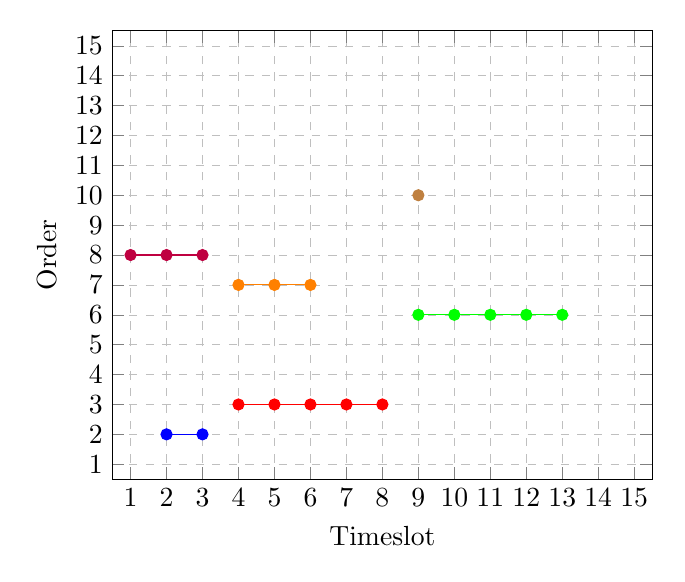
\begin{tikzpicture}
\begin{axis}[
    title={},
    xlabel={Timeslot},
    ylabel={Order},
    xmin=0.5, xmax=15.5, 
    ymin=0.5, ymax=15.5, 
    xtick={1,2,3,4,5,6,7,8,9,10,11,12,13,14,15},
    ytick={1,2,3,4,5,6,7,8,9,10,11,12,13,14,15},
    grid=both,
    grid style={line width=.1pt, draw=gray!10},
    major grid style={line width=.2pt, draw=gray!50},
    legend pos=north east,
    ymajorgrids=true,
    xmajorgrids=true,
    grid style=dashed,
]

% Order 2
\addplot[color=blue, mark=*] coordinates {(2, 2) (3, 2)};

% Order 3
\addplot[color=red, mark=*] coordinates {(4, 3) (5, 3) (6, 3) (7, 3) (8, 3)};

% Order 6
\addplot[color=green, mark=*] coordinates {(9, 6) (10, 6) (11, 6) (12, 6) (13, 6)};

% Order 7
\addplot[color=orange, mark=*] coordinates {(4, 7) (5, 7) (6, 7)};

% Order 8
\addplot[color=purple, mark=*] coordinates {(1, 8) (2, 8) (3, 8)};

% Order 10
\addplot[color=brown, mark=*] coordinates {(9, 10)};



\end{axis}
\end{tikzpicture}
\caption[Example of an approximated Schedule]{This schedule was created using the plain greedy implementation. It achieves a objective function value of 38.}
\label{fig:test}
\end{figure}
\section{Meta-heuristics}

\section{Parameter Tuning}

\end{document}
